%----------------------------------------------------------------------------------------
%	PACKAGES AND THEMES
%----------------------------------------------------------------------------------------

\documentclass{beamer}

\mode<presentation> {

% The Beamer class comes with a number of default slide themes
% which change the colors and layouts of slides. Below this is a list
% of all the themes, uncomment each in turn to see what they look like.

%\usetheme{default}
%\usetheme{AnnArbor}
%\usetheme{Antibes}
%\usetheme{Bergen}
%\usetheme{Berkeley}
%\usetheme{Berlin}
%\usetheme{Boadilla}
%\usetheme{CambridgeUS}
%\usetheme{Copenhagen}
%\usetheme{Darmstadt}
%\usetheme{Dresden}
%\usetheme{Frankfurt}
%\usetheme{Goettingen}
%\usetheme{Hannover}
%\usetheme{Ilmenau}
%\usetheme{JuanLesPins}
%\usetheme{Luebeck}
\usetheme{Madrid}
%\usetheme{Malmoe}
%\usetheme{Marburg}
%\usetheme{Montpellier}
%\usetheme{PaloAlto}
%\usetheme{Pittsburgh}
%\usetheme{Rochester}
%\usetheme{Singapore}
%\usetheme{Szeged}
%\usetheme{Warsaw}

% As well as themes, the Beamer class has a number of color themes
% for any slide theme. Uncomment each of these in turn to see how it
% changes the colors of your current slide theme.

%\usecolortheme{albatross}
%\usecolortheme{beaver}
%\usecolortheme{beetle}
%\usecolortheme{crane}
%\usecolortheme{dolphin}
%\usecolortheme{dove}
%\usecolortheme{fly}
%\usecolortheme{lily}
%\usecolortheme{orchid}
%\usecolortheme{rose}
%\usecolortheme{seagull}
%\usecolortheme{seahorse}
%\usecolortheme{whale}
%\usecolortheme{wolverine}

%\setbeamertemplate{footline} % To remove the footer line in all slides uncomment this line
\setbeamertemplate{footline}[page number] % To replace the footer line in all slides with a simple slide count uncomment this line

\setbeamertemplate{navigation symbols}{} % To remove the navigation symbols from the bottom of all slides uncomment this line
}

\usepackage{graphicx} % Allows including images
\usepackage{booktabs} % Allows the use of \toprule, \midrule and \bottomrule in tables
%\usepackage {tikz}
\usepackage{tkz-graph}
\GraphInit[vstyle = Shade]
\tikzset{
  LabelStyle/.style = { rectangle, rounded corners, draw,
                        minimum width = 2em, fill = yellow!50,
                        text = red, font = \bfseries },
  VertexStyle/.append style = { inner sep=5pt,
                                font = \normalsize\bfseries},
  EdgeStyle/.append style = {->, bend left} }
\usetikzlibrary {positioning}
%\usepackage {xcolor}
\definecolor {processblue}{cmyk}{0.96,0,0,0}
%----------------------------------------------------------------------------------------
%	TITLE PAGE
%----------------------------------------------------------------------------------------

\title[Short title]{ Learning English } % The short title appears at the bottom of every slide, the full title is only on the title page

\author{Swayam Jena} % Your name
\titlegraphic{
\includegraphics[width=2cm]{image/ktgs.jpg}}
\institute[KT Global School] % Your institution as it will appear on the bottom of every slide, may be shorthand to save space
{
KT Global School\\ % Your institution for the title page
\medskip
}
\date{\today} % Date, can be changed to a custom date

\begin{document}

\begin{frame}
\titlepage % Print the title page as the first slide
\end{frame}

\begin{frame}
\frametitle{Table of contents} % Table of contents slide, comment this block out to remove it
\tableofcontents % Throughout your presentation, if you choose to use \section{} and \subsection{} commands, these will automatically be printed on this slide as an overview of your presentation
\end{frame}

%----------------------------------------------------------------------------------------
%	PRESENTATION SLIDES
%----------------------------------------------------------------------------------------

%------------------------------------------------

\section{Parts of a Sentence}
\begin{frame}{Parts of a Sentence:}
\centering
   \textbf{The subject and predicate:}
   \par
   \vspace{0.25in}
   In English, every sentence needs two parts. The subject and the predicate
   \par
   \vspace{0.2in}
   \textcolor{blue}{The cat} \textcolor{red}{runs down the lane}
   \par
   \vspace{0.2in}
   \textcolor{blue}{Subject}  \textcolor{red}{Predicate}
   \par
   \vspace{0.2in}
   The Subject and the Predicate must be in order
\end{frame}
\section{Nouns}
\begin{frame}{Nouns}
\centering
  \textbf{ Noun Categories} \\
  \begin{table}[]
      \centering
      \begin{tabular}{|c|c|c|c|c|}
      \hline
\textbf{ Person }& \textbf{Place} & \textbf{Thing} & \textbf{Animal} & \textbf{Feeling}  \\
\hline fireman, bus & New York & pencil & dog, bird, & Love, hate,\\
driver, man & America & apple, desk & cat & anger\\
 & space & & &\\
 \hline
      \end{tabular}
      \caption{Noun Catagories}
      \label{tab:placeholder}
  \end{table}
\end{frame}

\begin{frame}{Nouns}
\centering
\textbf{Singular or Plural}\\
\begin{Table}
\centering
\begin{tabular}{|c|c|c|}
\hline
\textbf{Singular} & \textbf{Plural} & \textbf{Rule}\\
\hline
Apple & Apples & Add 's'\\
\hline
Fox & Foxes & Add 'es\\
\hline
Cherry & Cherries & Drop 'y' and add 'ies'\\
\hline
\end{tabular}
    
\end{Table}

\end{frame}

\section{Verbs}
\begin{frame} {Verbs}
\centering 
\textbf{What is a verb?}\\
\vspace{0.2in}
A \textcolor{red}{verb} is used to describe an action, state, or occurrence. The verb is the main part of the \textcolor{red}{predicate}.\\
\vspace{0.2in}
The cat \textcolor{red}{runs} down the lane.\\
\vspace{0.2in}
"Runs" is the \textcolor{red}{verb}.\\
\vspace{0.2in}
This is the action the cat (\textcolor{blue}{subject}) is doing.

\end{frame}
\begin{frame}{Verb}
\centering 
\textbf{Verb: Past, Present, and Future}\\
Verbs tell when an action takes place. The past, present, or future.\\ There are specific rules for each.\\
\begin{table}[]
    \centering
    \begin{tabular}{|c|c|}
    \hline
Verb - To talk & General Rule\\
\hline
Past : Talked & Add 'ed'\\
\hline
Present : Talks, Talk & Unchanged / add 's' or 'es'\\
\hline
Future : Will Talk & Add 'will' before the verb\\ 
\hline


    \end{tabular}
    \caption{*Not every verb follow these rules.}
    \label{tab:placeholder}
\end{table}

    
\end{frame}
\begin{frame}{Verb}
\centering
\textbf{Types of verb : Action}\\ 
\vspace{0.2in}
\textcolor{red}{Verbs} have many uses. One common verb type is an \textcolor{red}{action verb}.\\
\vspace{0.2in}
An \textcolor{red}{action verb} shows what the action the subject is doing.\\
\vspace{0.2in}
The cats \textcolor{red}{run} down the lane.\\
\vspace{0.2in}
"Runs" is the \textcolor{red}{action verb}. The action the cat is doing is running.
    
\end{frame}
\begin{frame}{Verb}
\centering
\textbf{Types of Verbs : Helping Verbs, Modal Verbs, and More}\\ 
\vspace{0.2in}
\textbf{Helping Verbs}\\
\vspace{0.2in}
She \textcolor{brown}{is} \textcolor{red}{standing} on the table.\\
\vspace{0.2in}
\textcolor{brown}{is} + \textcolor{red}{standing} (\textcolor{brown}{helping verb} + \textcolor{red}{main verb})
\end{frame}
\begin{frame}{Verb}
\centering
\textbf{Modal Verbs}\\
\vspace{0.2in}
He \textcolor{violet}{could} \textcolor{red}{fly} in the morning.\\
\vspace{0.2in}
\textcolor{violet}{could} + \textcolor{red}{fly} (\textcolor{violet}{modal verb} + \textcolor{red}{main verb})\\
\vspace{0.2in}
*These are just a few forms verbs can take.
\section{English sentence-Linking and transitive verbs}
\end{frame}
\begin{frame}{English sentence-Linking and transitive verbs} 
\centering
We learned that an English sentence has a subject and a verb with an object. However, it's not quite that simple. There are sentences that can be made without, or even more than one object. In this lesson we will take a look the different types in detail. 

    
\end{frame}
\begin{frame}{English sentence-Linking and transitive verbs}
\centering
We will focus on 3 different types of sentences. The sentence is different due to verb. The 3 types of verbs are:\\
\vspace{0.2in}
\begin{itemize}
    \item Transitive verb (monotransitive and ditransitive)
    \item Intransitive verb
    \item Linking verb
\end{itemize}
    
\end{frame}
\begin{frame}{English sentence-Linking and Transitive verbs}
\centering
Transitive verbs are the sentences we began talking about. These are two types of transitive verb sentences.\\
\vspace{0.2in}
\textbf{\underline{Monotransitive sentences}}\\
\vspace{0.2in}
\textcolor{blue}{Subject} + \textcolor{red}{Verb} + \textcolor{red}{Object}\\
\vspace{0.2in}
\textbf{\underline{Ditransitive sentences:}}\\
\vspace{0.2in}
\textcolor{blue}{Subject} + \textcolor{red}{Verb} + \textcolor{purple}{Indirect Object} + \textcolor{red}{Direct Object}

    
\end{frame}
\begin{frame}{English sentence-Linking and Transitive verbs}
\centering
\textbf{\underline{Monotransitive sentences:}}\\ 
\vspace{0.2in}
\textcolor{blue}{Subject} + \textcolor{red}{Verb} + \textcolor{red}{Object}\\
\vspace{0.2in}
Sakshsam kicked the ball\\
\vspace{0.2in}
\textbf{\underline{Ditransitive sentences:}}\\
\vspace{0.2in}
\textcolor{blue}{Subject} + \textcolor{red}{Verb} + \textcolor{purple}{Indirect Object} + \textcolor{red}{Direct Object}\\
\vspace{0.2in}
Swayam gave Saksham the cake.
\end{frame}
\begin{frame}{English sentence-Linking and Transitive verbs}
\centering
\textbf{Direct objects} are the nouns or pronouns receiving the action, while the \textbf{indirect objects} are the nouns or pronouns affected by the action. \textbf{Indirect objects} are the recipients of the \textbf{direct objects}. An indirect object aneswers the question of to whom, for whom, or for what.\\
\vspace{0.2in}
\textcolor{blue}{Subject} + \textcolor{red}{Verb} + \textcolor{purple}{Indirect Object} + \textcolor{red}{Direct Object}\\
\vspace{0.2in}
Swayam gave saksham the cake.\\
\vspace{0.2in}
Swayam pitched Sai prasad the basketball.
\end{frame}
\begin{frame}{English sentence-Linking and transitive verbs}
\centering
Intransitive verbs have no real object. Their action is not transferred from the subject to an object.\\
\vspace{0.2in}
\textbf{\underline{Intransitive sentences:}}\\
\vspace{0.2in}
\textcolor{blue}{Subject} + \textcolor{red}{Verb} + \textcolor{red}{(Preprositional Phrase)}\\
\vspace{0.2in}
\textcolor{blue}{She} \textcolor{red}{cried.}\\
\vspace{0.2in}
\textcolor{blue}{She} \textcolor{red}{cried (at home).}    
\end{frame}
\begin{frame}{English sentence-Linking and Transitive verbs.}
\centering
We can follow intransitive verbs with other words telling us \italic{how, where or when,} but isn't really the object:\\
\vspace{0.2in}
\textcolor{blue}{He} \textcolor{red}{slept after dinner.}\\
\vspace{0.2in}
\textcolor{blue}{Our car} \textcolor{red}{blew down the street.}\\   
\end{frame}
\begin{frame}{English sentence-Linking and Transitive verbs}
\centering
Linking verbs link two parts of a sentence. They link the subject tota noun or adjective called the subject complement.\\
\vspace{0.2in}
\textcolor{blue}{Subject} + \textcolor{red}{Verb} + \textcolor{red}{Subject Complement}\\
\vspace{0.2in}
\textcolor{blue}{Ranu} \textcolor{red}{is a doctor.} \\  
\end{frame}
\section{English sentence-Adjectives, Adverbs, and More}
\begin{frame}{Parts of an sentence-Adjectives, Adverbs, and More}
\centering
\textbf{The Other Words}\\
\vspace{0.2in}
\textcolor{blue}{Nouns} and \textcolor{red}{verbs} are the basic building blocks.\\
\vspace{0.2in}
\underline{The big} \textcolor{blue}{cat} \textcolor{red}{runs} \underline{down the} \textcolor{blue}{lane} \underline{quickly}.\\
\vspace{0.2in}
We use adverbs, adjectives, and determiners to give more imformation.\\   
\end{frame}
\begin{frame} {Parts of an sentence-Adjectives, Adverbs, and More}
\centering
\textbf{Adjectives and Adverbs : Adding detail to nouns and verbs}\\
\vspace{0.2in}
\textbf{Adjectives} are words that describe a noun. This adds more detail to the noun.\\
\vspace{0.2in}
The cat runs down the lane.\\
\vspace{0.2in}
The \textcolor{green}{brown} cat runs down the \textcolor{green}{old} lane.\\   
\end{frame}
\begin{frame}{Parts of an sentence-Adjectives, Adverbs, and More}
\centering
\textbf{Adjectives and Adverbs : Adding detail to nouns and verbs}\\
\vspace{0.2in}
\textbf{Adverbs} are words that describe a verb. This adds more detail to the verb.\\
\vspace{0.2in}
The cat runs down the lane.\\
\vspace{0.2in}
The cat runs \textcolor{orange}{quickly} down the lane.
\end{frame}
\begin{frame}{Parts of an sentence-Adjectives, Adverbs, and More}
\centering
\textbf{Determiniters : Adding even more detail}\\
\vspace{0.2in}
Determiners are words that allow us to add even more detail to our sentences.\\
\vspace{0.2in}
We have many different types to demostrate amount, time, location, and many other things.\\
\end{frame}
\begin{frame}{Parts of a sentence-Adjectives, Adverbs, and More}
\centering
\textbf{Determiners : Adding even more detail}\\
\vspace{0.2in}
\textbf{Articles :} used to show specificity\\
\vspace{0.2in}
A, An, and The\\
\vspace{0.2in}
\textcolor{blue}{The} cat runs down \textcolor{blue}{the} lane.\\
\vspace{0.2in}
\textcolor{blue}{A} cat runs down \textcolor{blue}{a} lane.\\    
\end{frame}
\begin{frame}{Parts of an sentence-Adjectives, Adverbs, and More}
\centering
\textbf{Determiners : Adding even more detail}\\
\vspace{0.2in}
\textbf{Demonstratives :} used to show which objects are being talked about\\
\vspace{0.2in}
This, That, These, Those\\
\vspace{0.2in}
\textcolor{green}{This} ball is red, \textcolor{green}{that} ball is blue.\\    
\end{frame}
\begin{frame}{Parts of a sentence-Adjectives, Adverbs, and More}
\centering
\textbf{Determiners : Adding even more detail}\\
\vspace{0.2in}
\textbf{Quantifiers :} tell how much or how many\\
\vspace{0.2in}
Some, many, a lot of, few\\
\vspace{0.2in}
\textcolor{brown}{Many} people eat meat, but \textcolor{brown}{some} do not.


    
\end{frame}
\begin{frame}{Parts of an sentence-Adjectives, Adverbs, and More}
\centering
\textbf{Determiners : Adding even more detail}\\
\vspace{0.2}
\textbf{Distributives :} used to talk about objects in a group\\
\vspace{0.2in}
Each, Every\\
\vspace{0.2in}
\textcolor{blue}{Every} student will take test, \textcolor{blue}{Each} student will have different questions. 


    
\end{frame}
\section{Parts of a sentence-Prepositions}
\begin{frame}{Parts of an sentence-Prepositions}
\centering
\textbf{What are prepositions?}\\
\vspace{0.2in}
Prepositions are words that we use to show the relationship between other words. They give us imformation about time, location, or movement.\\
\vspace{0.3in}
The cat runs \textcolor{blue}{down} the lane.\\
\vspace{0.2in}
The cat runs \textcolor{blue}{on} the lane.   
\end{frame}
\begin{frame}{Parts of an sentence-Prepositions}
\centering
\textbf{Prepositional Phrase}\\
\vspace{0.2in}
A prepositional phrase is a preposition with the object it belongs to\\
\vspace{0.2in}
The cat runs \textcolor{blue}{down} the lane.\\
\vspace{0.2in}
\textcolor{blue}{down the lane}\\
\vspace{0.2in}
The cat runs \textcolor{blue}{on} the lane.\\
\vspace{0.2in}
\textcolor{blue}{on the lane}\\   
\end{frame}
\begin{frame}{Parts of an sentence-Prepositions}
\centering
\textbf{Types of Prepositions}\\
\vspace{0.2in}
\underline{Time(when)}\\
I start school \textcolor{blue}{in} September.\\
\vspace{0.2in}
\underline{Place(where)}\\
She jumped \textcolor{blue}{on} the table.\\
\vspace{0.2in}
\underline{Movement(how)}\\
He walks \textcolor{blue}{to} work.\\
\vspace{0.2in}
. In, to, and on are very common prepositions. However, there are many more.     
\end{frame}
\begin{frame}{Parts of an sentence-Prepositions}
\centering
\vspace{0.5in}
 \begin{tabular}{|c|c|c|}
 \hline
 Time & Movement & Location\\
 \hline
 On & Info & Above\\
 Form & Toward & Over\\
 During & Down & Under\\
 By & Along & Between\\
 \hline
 \end{tabular}
\end{frame}
\section{Parts of a sentence-Conjunctions}
\begin{frame}{Parts of a sentence-Conjuctions}
\centering
\textbf{What are Conjuctions?}\\
\vspace{0.2in}
A conjuction is a word used to connect clauses or sentences\\
\vspace{0.2in}
I have a dog. I have a cat.\\
\vspace{0.2in}
I have a dog \textcolor{purple}{and} a cat.\\    
\end{frame}
\begin{frame}{Parts of a sentence-Conjuctions}
\centering
\textbf{Types of conjuctions}\\
\vspace{0.2in}
There are 3 main types of conjuctions.\\
\vspace{0.2in}
\textcolor{purple}{Coordinating :} joins words, phrases that are similar\\
\vspace{0.2in}
\textcolor{purple}{Suboarding :} show a relationship between two situations\\
\vspace{0.2in}
\textcolor{purple}{Correlative :} pairs of conjuctions used to join words, phrases that are similar\\    
\end{frame}
\begin{frame}{Parts of a sentence-Conjuctions}
\centering
\textbf{Types of Conjuctions : Coordinating}\\
\vspace{0.2in}
\textcolor{purple}{Coordinating conjuctions} join words and phrases that are similar.\\
\vspace{0.2in}
I like dogs. I like cats.\\
\vspace{0.2in}
I like dogs \textcolor{purple}{and} cats.\\
\vspace{0.2in}
These conjuctions can easily be remembered using the word FANBOYS (for, and, nor, but, or, yet, so)\\    
\end{frame}
\begin{frame}{Parts of a sentence-Conjuctions}
\centering
\textbf{Types of Conjuctions : Suboardinating}\\
\vspace{0.2in}
\textcolor{purple}{Suboardinating conjuctions} show a relationship between two situations.\\
\vspace{0.2in}
It was hot outside. The ice cream melted.\\
\vspace{0.2in}
The ice cream melted since it was hot outside.\\
\vspace{0.2in}
Since it was hot outside, the ice cream melted.\\
\vspace{0.2in}
\textbf{Some common suboardinating conjuctions are:} than, rather than, whether, as much as, wheras, which, whichever, after, as soon as, as long as, before, by the time, now that, once, since, till, untill, when, whenever, while, through, altrough, even through\\
\end{frame}
 \begin{frame}{Parts of a sentence-Conjuctions}
 \centering
 \textbf{Types of Conjuctions : Correlative}\\
 \vspace{0.2in}
 \textcolor{purple}{Correlative conjuctions} are pairs of conjuctions used to join words, phrases that are similar.\\
 \vspace{0.2in}
 I don't like pizza. I don't like pasta.\\
 \vspace{0.2in}
 I like \textcolor{purple}{neither} pizza \textcolor{purple}{nor} pasta.\\
 \vspace{0.2in}
 Some common correlative conjunctions are : either...or, neither...nor, not only...but also     
 \end{frame}
\section{Simple present tense}
\begin{frame}{Simple present tense}
\centering
\begin{tabular}{|c|c|c|}
\hline
 & Singular & Plural\\
\hline
1st Person & I eat & we eat\\
\hline
2nd person & you eat & you eat\\
\hline
3rd person & he/she/it eats & they eat\\
\hline
\end{tabular}    
\end{frame}
\begin{frame}{Simple present tense}
\centering
Simples present tense uses\\
\vspace{0.3in}
\begin{itemize}
\item[$\rightarrow$]  Routlines and habits\\
\item[$\rightarrow$]  Facts and truths\\
\item [$\rightarrow$] Scheduled events\\
\item[$\rightarrow$] Pernament situations or states\\
\item [$\rightarrow$] Instructions or directions\\  
\end{itemize}
\end{frame}
\begin{frame}{Simple present tense}
\centering
Routlines and habits\\
\vspace{0.2in}
The Simple present tense is used to talk about things you do regularly.\\
\vspace{0.4in}
I go to the gym every day.\\
She drinks coffee every morning.\\   
\end{frame}
\begin{frame}{Simple present tense}
\centering
Facts or truths\\
\vspace{0.2in}
The Simple present tense is used to state facts or truths that are always true.\\
\vspace{0.4in}
The earth orbits the sun.\\
Water bolls at 100 degree celslus.\\
\end{frame}
\begin{frame}{Simple present tense}
\centering
Schedules events\\
\vspace{0.2in}
The Simple present tense is used for events that are scheduled in the future, espicially with timetables or ltlneraries.\\
\vspace{0.2in}
The train leaves in 6 PM.\\
The meeting starts at 10 AM tomorrow.\\    
\end{frame}
\begin{frame}{Simple present tense}
\centering
Pernament situations or states\\
\vspace{0.2in}
The Simple present tense is used to describe pernament situations or states.\\
\vspace{0.2in}
He lives in New york.\\
She works as a teacher.    
\end{frame}
\begin{frame}{Simple present tense}
\centering
Instructions or directions\\
\vspace{0.2in}
The Simple present tense is used when giving instructions or directions.\\
\vspace{0.2in}
First you add the flour to the bowl.\\
You turn left at the traffic lights.\\    
\end{frame}    
\begin{frame}{Simple present tense}
\centering
Forming the Simple present tense\\
\vspace{0.3in}
\begin{itemize}
\item [$\rightarrow$]Positive sentences
\item[$\rightarrow$]Negative sentences
\item [$\rightarrow$]Questions    
\end{itemize}
\end{frame}
\begin{frame}{Simple present tense}
\centering
Positive sentences\\
\vspace{0.2in}
Use only the base form of the verb for subjects "I","you","he","she","it", and "they".\\
\vspace{0.2in}
For 3rd person singular subjects,"he","she", and "it", add "s" or "es" to the base form of the verb.\\
\vspace{0.3in}
Subject + Verb\\
\vspace{0.4in}
I work in an office.\\
She works in an office.\\    
\end{frame}
\begin{frame}{Simple present tense}
\centering
Negative sentences \\
\vspace{0.2in}
Use "do not" (don't) or "does not" (doesn't) before the base form of the verb.\\
\vspace{0.2in}
Subject + "do/does" + "not" + verb\\
\vspace{0.3in}
\begin{itemize}
\item[$\rightarrow$] "Do not" is used with "I","you","we" and "they".\\
\item[$\rightarrow$] "Does not" is used with 3rd person singular subjects, "he","she", and "it".\\
\end{itemize}
\centering
\vspace{0.4in}
I do not work in an office.\\
She does not work in an office.\\    
\end{frame}
\section{About me}
\begin{frame}{About me}
\centering
\textbf{Swayam Jena}\\
Grade:5\\
KT Global School\\
swayam.jena17@gmail.com\\
\begin{figure}
    \centering
    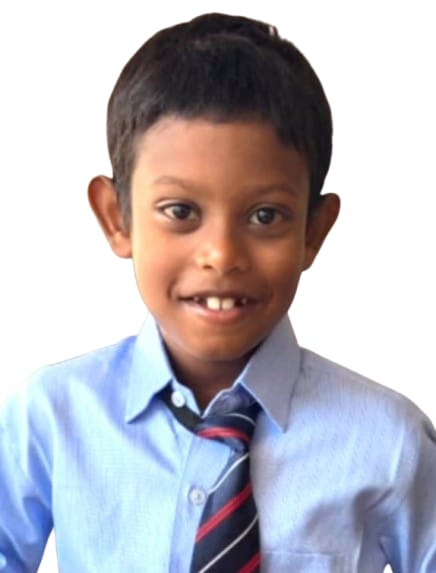
\includegraphics[scale=0.25]{image/swayam.jpeg}
    \caption{Swayam Jena}
    \label{fig:placeholder}
\end{figure}
    
\end{frame}

\begin{frame}
\Huge{\centerline{The End}}
\end{frame}

\end{document}